\documentclass[notes]{subfiles}
\begin{document}
	\addcontentsline{toc}{section}{2.6 - Rate of Change Graphs}
	\refstepcounter{section}
	\fancyhead[RO,LE]{\bfseries  \large \nameref{cs26}} 
	\fancyhead[LO,RE]{\bfseries  \currentname}
	\fancyfoot[C]{{}}
	\fancyfoot[RO,LE]{\large \thepage}	%Footer on Right \thepage is pagenumber
	\fancyfoot[LO,RE]{\large Chapter 2.6}


\section*{Rate of Change Graphs}\label{cs26}
	We will use the following terminology interchangeably:\showto{st}{\\}
	\begin{itemize}
		\item \showto{ins}{\fbox{slope graph}}\showto{st}{\blank{3}\\}
		\item \showto{ins}{\fbox{rate of change graph}}\showto{st}{\blank{3}\\}
		\item \showto{ins}{\fbox{derivative graph}}\showto{st}{\blank{3}\\}
	\end{itemize}
	The following information will be useful when constructing slope graphs:
		\begin{center}	
			\tabulinesep=3mm
			\begin{tabu}{ | X[.5,c] | X[c] | X[c] |}\hline
				\textbf{Derivative is}: & \textbf{Function graph is}: & \textbf{Slope graph is}:\\ \hline
						& & \\
				Positive	& & \\ 
				 		& & \\ \hline
				 		& & \\
				Zero 	& & \\ 
				 		& & \\ \hline
				 		& & \\
				Negative & & \\ 
						& & \\ \hline				
			\end{tabu}
		\end{center}
		
	Things to keep in mind when plotting the slope graph: \showto{st}{\\}
		\begin{itemize}
			\item \showto{ins}{\fbox{Horizontal tangents}}\showto{st}{\blank{3}} result in a max or min \emph{on the derivative graph}.\showto{st}{\\[10pt]}
			\item Derivatives may fail to exist at some points; there may be a \showto{ins}{\fbox{vertical asymptote}, \fbox{discontinuity}, \fbox{or corner}}\showto{st}{\blank{2}\\[15pt]\blank{5}.\\}
			\item The slope graph reports \showto{ins}{\fbox{slopes}}\showto{st}{\blank{1.5}} of the original graph; a negative slope results \showto{st}{\\[15pt]} in a \showto{ins}{\fbox{negative value}}\showto{st}{\blank{1.5}}, and a positive slope results in a \showto{ins}{\fbox{positive value}}\showto{st}{\blank{2}}.
		\end{itemize}
			\newpage
			
		\begin{ex}
			Sketch the rate of change graph for the function 
			\begin{center}
				\begin{tikzpicture}
					\begin{axis}[
						scale = 1.5,
						every tick label/.append style={font=\small},
						axis x line = middle,
						axis y line = middle,
			    			every axis y label/.style={at={(ticklabel cs:1.15)}},
			    			ytick = {0},
							y label style={at={(axis description cs:.2,1.15)},anchor=north},
			    			ylabel = {$f(x)$},
			    			ymin = -.5, ymax = 5,
		    				every axis x label/.style= {at ={(ticklabel cs:1)}},
		    				xtick = {1.13, 2.33, 3.53},
		    					x label style={at={(axis description cs:1.1,.1)},anchor=east},
		    				xlabel = {$x$},
		    				xmin = -1, xmax = 5
					]
						\addplot[thick, smooth,domain = -0.2:4.9] {.5*x^3-3.5*x^2+6*x+1.3};
						\coordinate (a1) at (1.13,4.33);
						\coordinate (a2) at (1.13,0);
						\coordinate (b1) at (2.33,2.6);
						\coordinate (b2) at (2.33,0);
						\coordinate (c1) at (3.53,0.86);
						\coordinate (c2) at (3.53,0);
					\end{axis}
					\draw[dashed] (a1)--(a2);
					\draw[dashed] (b1)--(b2);
					\draw[dashed] (c1)--(c2);
				\end{tikzpicture}	
			\end{center}
				\vs{1}
			\begin{center}
				\begin{tikzpicture}
					\begin{axis}[
						scale = 1.5,
						every tick label/.append style={font=\small},
						axis x line = middle,
						axis y line = middle,
			    			every axis y label/.style={at={(ticklabel cs:1.15)}},
			    			ytick = {0},
							y label style={at={(axis description cs:.2,1.15)},anchor=north},
			    			ylabel = {$f'(x)$},
			    			ymin = -.5, ymax = 5,
		    				every axis x label/.style= {at ={(ticklabel cs:1)}},
		    				xtick = {1.13, 2.33, 3.53},
		    					x label style={at={(axis description cs:1.1,.1)},anchor=east},
		    				xlabel = {$x$},
		    				xmin = -1, xmax = 5
					]
					\end{axis}
				\end{tikzpicture}
			\end{center}
		\end{ex}
			\vs{.5}
			\newpage
			
		\begin{ex}
			Sketch (and label) the slope graphs of the following functions:
		\begin{enumerate}[(a)]
			\item 
			\tabulinesep = .5in
			\begin{tabu}{X[l] X[.25,c] X[r]}
				\begin{tikzpicture}[x = .8cm, y = .8cm]
					\draw[->] (-3,0)--(6,0) node[right] {$x$};
					\draw[->] (0,-3)--(0,6) node[above] {$y$};
					\draw [<->,smooth, samples = 100, domain = -.5:6] plot (\x,{5./(1+exp(-(2.*\x-5)))});
					\fill (2.5,2.5) circle (.1);
					\draw[dashed] (2.5,2.5)--(2.5,0);
					\draw (2.5,2pt)--(2.5,-2pt) node [anchor = north] {\footnotesize $a$};
				\end{tikzpicture} 
				& &
				\begin{tikzpicture}[x = .8cm, y = .8cm]
					\draw[->] (-3,0)--(6,0) node[right] {$x$};
					\draw[->] (0,-3)--(0,6) node[above] {$y$};
					\draw [<->,smooth, samples = 100, domain = -.5:6] plot (\x,{-\x + 5});
				\end{tikzpicture}
					\\[15pt] %First row graphs
				\begin{tikzpicture}[x = .8cm, y = .8cm]
					\draw[->] (-3,0)--(6,0);
					\draw[->] (0,-3)--(0,6);
					\draw (2.5,2pt)--(2.5,-2pt) node [anchor = north] {\footnotesize $a$};
				\end{tikzpicture} 
				& & 
				\begin{tikzpicture}[x = .8cm, y = .8cm]
					\draw[->] (-3,0)--(6,0);
					\draw[->] (0,-3)--(0,6);
				\end{tikzpicture}
					\\ %First row slope graphs
			\end{tabu}
				\vs{1}
				\newpage
			
			\item
			\tabulinesep = .5in
			\begin{tabu}{X[l] X[.25,c] X[r]}
				\begin{tikzpicture}[x = .8cm, y = .8cm]
					\draw[->] (-3,0)--(6,0) node[right] {$x$};
					\draw[->] (0,-3)--(0,6) node[above] {$y$};
					\draw [<->,smooth, samples = 100, domain = 0.:5] plot (\x, {(\x-2.5)^2-1});
					\fill (2.5,-1) circle (.1);
					\draw[dashed] (2.5,-1)--(2.5,0);
					\draw (2.5,1pt)--(2.5,-2pt) node [anchor = south] {\footnotesize $a$};
				\end{tikzpicture} 
				& &
				\begin{tikzpicture}[x = .8cm, y = .8cm]
					\draw[->] (-3,0)--(6,0) node[right] {$x$};
					\draw[->] (0,-3)--(0,6) node[above] {$y$};
					\draw [<->,smooth, samples = 100, domain = 0.3:5.] plot (\x,{2*ln(\x)});
				\end{tikzpicture}
					\\[15pt] %Second row graphs
				
				\begin{tikzpicture}[x = .8cm, y = .8cm]
					\draw[->] (-3,0)--(6,0);
					\draw[->] (0,-3)--(0,6);
					\draw (2.5,1pt)--(2.5,-2pt) node [anchor = south] {\footnotesize $a$};
				\end{tikzpicture}
				& & 
				 \begin{tikzpicture}[x = .8cm, y = .8cm]
					\draw[->] (-3,0)--(6,0);
					\draw[->] (0,-3)--(0,6);
				\end{tikzpicture}
					\\ %Second row slope graphs
			\end{tabu}
				\vs{1}
				\newpage
				
			\item
			\tabulinesep = .5in	
			\begin{tabu}{X[l] X[.25,c] X[r]}
				\begin{tikzpicture}[x = .8cm, y = .8cm]
					\draw[->] (-3,0)--(3,0) node[right] {$x$};
					\draw[->] (0,-3)--(0,6) node[above] {$y$};
					\draw [<->,smooth,samples = 100, domain = -2.5:2.5] plot (\x,{10*(\x)*exp(-(1.2*(\x))^2)+.5});
					\fill (.6,4) circle (.1);
					\fill (-.6,-3) circle (.1);
					\fill (0,0) circle (.1);
					\draw (.3,-.2) node {\footnotesize $c$};
					\draw [dashed] (.6,4)--(.6,0);
					\draw [dashed] (-.6,-3)--(-.6,0);
					\draw (.6,2pt)--(.6,-2pt) node [anchor = north] {\footnotesize $b$};
					\draw (-.6,-2pt)--(-.6,2pt) node [anchor = south] {\footnotesize $a$};
				\end{tikzpicture}
				& &
				\begin{tikzpicture}[x = .8cm, y = .8cm]
					\draw[->] (-3,0)--(3,0) node[right] {$x$};
					\draw[->] (0,-3)--(0,6) node[above] {$y$};
					\draw[<->,smooth,samples = 100, domain = -2:2] plot (\x,{0.5*(\x)^4-(\x)^2+1});
					\fill (-1,.5) circle (.1);
					\fill (1,.5) circle (.1);
					\fill (0,1) circle (.1);
					\draw [dashed] (-1.,.5)--(-1.,0.);
					\draw [dashed] (1.,.5)--(1.,0.);
					\draw (-1.,2pt)--(-1.,-2pt) node[anchor = north] {\footnotesize $a$};
					\draw (1.,2pt)--(1.,-2pt) node[anchor = north] {\footnotesize $c$};
					\draw (0.15,0.1) node[anchor = north] {\footnotesize $b$};
				\end{tikzpicture} 
					\\[15pt] %Third row graphs
				\begin{tikzpicture}[x = .8cm, y = .8cm]
					\draw[->] (-3,0)--(6,0);
					\draw[->] (0,-3)--(0,6);
					\draw (.6,2pt)--(.6,-2pt) node [anchor = north] {\footnotesize $b$};
					\draw (-.6,2pt)--(-.6,-2pt) node [anchor = north] {\footnotesize $a$};
					\draw (.3,-.2) node {\footnotesize $c$};
				\end{tikzpicture}
				& &
				\begin{tikzpicture}[x = .8cm, y = .8cm]
					\draw[->] (-3,0)--(6,0);
					\draw[->] (0,-3)--(0,6);
					\draw (-1.,2pt)--(-1.,-2pt) node[anchor = north] {\footnotesize $a$};
					\draw (1.,2pt)--(1.,-2pt) node[anchor = north] {\footnotesize $c$};
					\draw (0.15,0.1) node[anchor = north] {\footnotesize $b$};
				\end{tikzpicture}
				\\ %Third row slope graphs
			\end{tabu}
		\end{enumerate}
		\end{ex}
			\vs{1}
			\newpage
			
		\begin{ex} 
			The figure below shows the membership in a campus organization during its first year.  Round all answers to the nearest member. \\[10pt]
			\begin{center}
				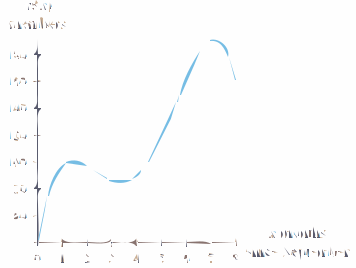
\includegraphics[scale = 1.5]{./img/sec26-1.png}
			\end{center}

			\begin{enumerate}[(a)]
				\item Estimate the average rate of change of membership from September through May.
					\vs{1}
				\item Estimate the instantaneous rate of change in October, December, and April.
					\vs{1}
				\item Sketch a rate-of-change graph for membership.  Label both axes.
					\vs{2}
					\newpage
			\end{enumerate}

		\end{ex}
			\newpage
		\begin{ex}
			The figure below shows cattle prices (for choice of 450-pound steer calves) from October 1994 through May 1995.\\[10pt]
			\begin{center}
				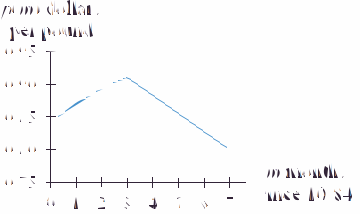
\includegraphics[scale = 1.5]{./img/sec26-2.png}
			\end{center}
			\begin{enumerate}[(a)]
				\item For which input value does the derivative fail to exist?  Give a clear, mathematical reason why.
					\vs{.5}
				\item Sketch a slope graph of $p$.  Label both axes.
					\vs{2}
			\end{enumerate}
		\end{ex}
			\newpage
			
		\begin{ex}
			Sketch the slope graph of a function $f$ with input $t$ that meets the following criteria:
				\begin{itemize}
					\item $f(-2) = 5$
					\item the slope is positive for $t < 2$
					\item the slope is negative for $t > 2$
					\item $f'(2)$ does not exist
				\end{itemize}
		\end{ex}
			\vs{1}
			
		\begin{ex}
			Sketch the slope graph of a function $g$ with input $x$ that meets these criteria:\\[5pt]
				\begin{tabular}{cc}
				\begin{minipage}{3.5in}
				\begin{itemize}
					\item $g(3)$ does not exist
					\item $g'(0) = -4$
					\item $g'(x) < 0$ for $x < 3$
					\item $g$ is concave down for $x < 3$
				\end{itemize}
				\end{minipage}
				\begin{minipage}{3.5in}
				\begin{itemize}
					\item $g'(x) < 0$ for $x > 3$
					\item $g$ is concave up for $x > 3$
					\item $\ds \lim_{x\to 3^+} g(x) \to \infty$
					\item $\ds \lim_{x\to 3^-} g(x) \to -\infty$
				\end{itemize}
				\end{minipage}
				\end{tabular}
		\end{ex}
			\vs{1}
\end{document}